\documentclass[11pt,compress,t,notes=noshow, aspectratio=169, xcolor=table]{beamer}

\usepackage{../../style/lmu-lecture}
% Defines macros and environments
\usepackage[]{graphicx}
\usepackage[]{color}
% maxwidth is the original width if it is less than linewidth
% otherwise use linewidth (to make sure the graphics do not exceed the margin)
\makeatletter
\def\maxwidth{ %
\ifdim\Gin@nat@width>\linewidth
\linewidth
\else
\Gin@nat@width
\fi
}
\makeatother
%\usepackage[fontsize=10.5pt]{scrextend}
\definecolor{ggred}{rgb}{0.973, 0.463, 0.427}
\definecolor{ggblue}{rgb}{0, 0.749, 0.769}
\definecolor{fgcolor}{rgb}{0.345, 0.345, 0.345}
\newcommand{\hlnum}[1]{\textcolor[rgb]{0.686,0.059,0.569}{#1}}%
\newcommand{\hlstr}[1]{\textcolor[rgb]{0.192,0.494,0.8}{#1}}%
\newcommand{\hlcom}[1]{\textcolor[rgb]{0.678,0.584,0.686}{\textit{#1}}}%
\newcommand{\hlopt}[1]{\textcolor[rgb]{0,0,0}{#1}}%
\newcommand{\hlstd}[1]{\textcolor[rgb]{0.345,0.345,0.345}{#1}}%
\newcommand{\hlkwa}[1]{\textcolor[rgb]{0.161,0.373,0.58}{\textbf{#1}}}%
\newcommand{\hlkwb}[1]{\textcolor[rgb]{0.69,0.353,0.396}{#1}}%
\newcommand{\hlkwc}[1]{\textcolor[rgb]{0.333,0.667,0.333}{#1}}%
\newcommand{\hlkwd}[1]{\textcolor[rgb]{0.737,0.353,0.396}{\textbf{#1}}}%
\newcommand{\predvar}{Var\left[\hat{f}(\xv)\right]}
\let\hlipl\hlkwb

\usepackage{pdfpages}
\usepackage{framed}
\makeatletter
\newenvironment{kframe}{%
\def\at@end@of@kframe{}%
\ifinner\ifhmode%
\def\at@end@of@kframe{\end{minipage}}%
\begin{minipage}{\columnwidth}%
\fi\fi%
\def\FrameCommand##1{\hskip\@totalleftmargin \hskip-\fboxsep
\colorbox{shadecolor}{##1}\hskip-\fboxsep
% There is no \\@totalrightmargin, so:
\hskip-\linewidth \hskip-\@totalleftmargin \hskip\columnwidth}%
\MakeFramed {\advance\hsize-\width
\@totalleftmargin\z@ \linewidth\hsize
\@setminipage}}%
{\par\unskip\endMakeFramed%
\at@end@of@kframe}
\makeatother

\definecolor{shadecolor}{rgb}{.97, .97, .97}
\definecolor{messagecolor}{rgb}{0, 0, 0}
\definecolor{warningcolor}{rgb}{1, 0, 1}
\definecolor{errorcolor}{rgb}{1, 0, 0}
\newenvironment{knitrout}{}{} % an empty environment to be redefined in TeX

\usepackage{alltt}
\newcommand{\SweaveOpts}[1]{}  % do not interfere with LaTeX
\newcommand{\SweaveInput}[1]{} % because they are not real TeX commands
\newcommand{\Sexpr}[1]{}       % will only be parsed by R

\usepackage[english]{babel}
\usepackage[utf8]{inputenc}

\usepackage[export]{adjustbox}
\usepackage{dsfont}
\usepackage{verbatim}
\usepackage{amsmath}
\usepackage{amsfonts}
\usepackage{bm}
\usepackage{csquotes}
\usepackage{multirow}
\usepackage{longtable}
\usepackage{booktabs}
\usepackage{enumerate}
\usepackage[absolute,overlay]{textpos}
\usepackage{psfrag}
\usepackage{algorithm}
\usepackage{algpseudocode}
\usepackage{eqnarray}
\usepackage{arydshln}
\usepackage{tabularx}
\usepackage{placeins}
\usepackage{tikz}
\usepackage{setspace}
\usepackage{colortbl}
\usepackage{mathtools}
\usepackage{wrapfig}
\usepackage{bm}
\usepackage[backend=biber]{biblatex}

\usetikzlibrary{tikzmark, shapes,arrows,automata,positioning,calc,chains,trees,  shadows, decorations.pathreplacing}
\tikzset{
%Define standard arrow tip
>=stealth',
%Define style for boxes
punkt/.style={
rectangle,
rounded corners,
draw=black, very thick,
text width=6.5em,
minimum height=2em,
text centered},
% Define arrow style
pil/.style={
->,
thick,
shorten <=2pt,
shorten >=2pt,}
}

\usepackage{subfig}

\usepackage{bbm}
%\newcommand\hmmax{0}
%\newcommand\bmmax{0}
% basic latex stuff
\newcommand{\pkg}[1]{{\fontseries{b}\selectfont #1}} %fontstyle for R packages
\newcommand{\lz}{\vspace{0.5cm}} %vertical space
\newcommand{\dlz}{\vspace{1cm}} %double vertical space
\newcommand{\oneliner}[1] % Oneliner for important statements
{\begin{block}{}\begin{center}\begin{Large}#1\end{Large}\end{center}\end{block}}

% Latexmath Notation
% math spaces
\ifdefined\N                                                                
\renewcommand{\N}{\mathds{N}} % N, naturals
\else \newcommand{\N}{\mathds{N}} \fi 
\newcommand{\Z}{\mathds{Z}} % Z, integers
\newcommand{\Q}{\mathds{Q}} % Q, rationals
\newcommand{\R}{\mathds{R}} % R, reals
\ifdefined\C 
  \renewcommand{\C}{\mathds{C}} % C, complex
\else \newcommand{\C}{\mathds{C}} \fi
\newcommand{\continuous}{\mathcal{C}} % C, space of continuous functions
\newcommand{\M}{\mathcal{M}} % machine numbers
\newcommand{\epsm}{\epsilon_m} % maximum error

% counting / finite sets
\newcommand{\setzo}{\{0, 1\}} % set 0, 1
\newcommand{\setmp}{\{-1, +1\}} % set -1, 1
\newcommand{\unitint}{[0, 1]} % unit interval

% basic math stuff
\newcommand{\xt}{\tilde x} % x tilde
\newcommand{\argmax}{\operatorname{arg\,max}} % argmax
\newcommand{\argmin}{\operatorname{arg\,min}} % argmin
\newcommand{\argminlim}{\mathop{\mathrm{arg\,min}}\limits} % argmax with limits
\newcommand{\argmaxlim}{\mathop{\mathrm{arg\,max}}\limits} % argmin with limits  
\newcommand{\sign}{\operatorname{sign}} % sign, signum
\newcommand{\I}{\mathbb{I}} % I, indicator
\newcommand{\order}{\mathcal{O}} % O, order
\newcommand{\pd}[2]{\frac{\partial{#1}}{\partial #2}} % partial derivative
\newcommand{\floorlr}[1]{\left\lfloor #1 \right\rfloor} % floor
\newcommand{\ceillr}[1]{\left\lceil #1 \right\rceil} % ceiling

% sums and products
\newcommand{\sumin}{\sum\limits_{i=1}^n} % summation from i=1 to n
\newcommand{\sumim}{\sum\limits_{i=1}^m} % summation from i=1 to m
\newcommand{\sumjn}{\sum\limits_{j=1}^n} % summation from j=1 to p
\newcommand{\sumjp}{\sum\limits_{j=1}^p} % summation from j=1 to p
\newcommand{\sumik}{\sum\limits_{i=1}^k} % summation from i=1 to k
\newcommand{\sumkg}{\sum\limits_{k=1}^g} % summation from k=1 to g
\newcommand{\sumjg}{\sum\limits_{j=1}^g} % summation from j=1 to g
\newcommand{\meanin}{\frac{1}{n} \sum\limits_{i=1}^n} % mean from i=1 to n
\newcommand{\meanim}{\frac{1}{m} \sum\limits_{i=1}^m} % mean from i=1 to n
\newcommand{\meankg}{\frac{1}{g} \sum\limits_{k=1}^g} % mean from k=1 to g
\newcommand{\prodin}{\prod\limits_{i=1}^n} % product from i=1 to n
\newcommand{\prodkg}{\prod\limits_{k=1}^g} % product from k=1 to g
\newcommand{\prodjp}{\prod\limits_{j=1}^p} % product from j=1 to p

% linear algebra
\newcommand{\one}{\boldsymbol{1}} % 1, unitvector
\newcommand{\zero}{\mathbf{0}} % 0-vector
\newcommand{\id}{\boldsymbol{I}} % I, identity
\newcommand{\diag}{\operatorname{diag}} % diag, diagonal
\newcommand{\trace}{\operatorname{tr}} % tr, trace
\newcommand{\spn}{\operatorname{span}} % span
\newcommand{\scp}[2]{\left\langle #1, #2 \right\rangle} % <.,.>, scalarproduct
\newcommand{\mat}[1]{\begin{pmatrix} #1 \end{pmatrix}} % short pmatrix command
\newcommand{\Amat}{\mathbf{A}} % matrix A
\newcommand{\Deltab}{\mathbf{\Delta}} % error term for vectors

% basic probability + stats
\renewcommand{\P}{\mathds{P}} % P, probability
\newcommand{\E}{\mathds{E}} % E, expectation
\newcommand{\var}{\mathsf{Var}} % Var, variance
\newcommand{\cov}{\mathsf{Cov}} % Cov, covariance
\newcommand{\corr}{\mathsf{Corr}} % Corr, correlation
\newcommand{\normal}{\mathcal{N}} % N of the normal distribution
\newcommand{\iid}{\overset{i.i.d}{\sim}} % dist with i.i.d superscript
\newcommand{\distas}[1]{\overset{#1}{\sim}} % ... is distributed as ...

% machine learning
\newcommand{\Xspace}{\mathcal{X}} % X, input space
\newcommand{\Yspace}{\mathcal{Y}} % Y, output space
\newcommand{\nset}{\{1, \ldots, n\}} % set from 1 to n
\newcommand{\pset}{\{1, \ldots, p\}} % set from 1 to p
\newcommand{\gset}{\{1, \ldots, g\}} % set from 1 to g
\newcommand{\Pxy}{\mathbb{P}_{xy}} % P_xy
\newcommand{\Exy}{\mathbb{E}_{xy}} % E_xy: Expectation over random variables xy
\newcommand{\xv}{\mathbf{x}} % vector x (bold)
\newcommand{\xtil}{\tilde{\mathbf{x}}} % vector x-tilde (bold)
\newcommand{\yv}{\mathbf{y}} % vector y (bold)
\newcommand{\xy}{(\xv, y)} % observation (x, y)
\newcommand{\xvec}{\left(x_1, \ldots, x_p\right)^\top} % (x1, ..., xp) 
\newcommand{\Xmat}{\mathbf{X}} % Design matrix
\newcommand{\allDatasets}{\mathds{D}} % The set of all datasets
\newcommand{\allDatasetsn}{\mathds{D}_n}  % The set of all datasets of size n 
\newcommand{\D}{\mathcal{D}} % D, data
\newcommand{\Dn}{\D_n} % D_n, data of size n
\newcommand{\Dtrain}{\mathcal{D}_{\text{train}}} % D_train, training set
\newcommand{\Dtest}{\mathcal{D}_{\text{test}}} % D_test, test set
\newcommand{\xyi}[1][i]{\left(\xv^{(#1)}, y^{(#1)}\right)} % (x^i, y^i), i-th observation
\newcommand{\Dset}{\left( \xyi[1], \ldots, \xyi[n]\right)} % {(x1,y1)), ..., (xn,yn)}, data
\newcommand{\defAllDatasetsn}{(\Xspace \times \Yspace)^n} % Def. of the set of all datasets of size n 
\newcommand{\defAllDatasets}{\bigcup_{n \in \N}(\Xspace \times \Yspace)^n} % Def. of the set of all datasets 
\newcommand{\xdat}{\left\{ \xv^{(1)}, \ldots, \xv^{(n)}\right\}} % {x1, ..., xn}, input data
\newcommand{\ydat}{\left\{ \yv^{(1)}, \ldots, \yv^{(n)}\right\}} % {y1, ..., yn}, input data
\newcommand{\yvec}{\left(y^{(1)}, \hdots, y^{(n)}\right)^\top} % (y1, ..., yn), vector of outcomes
\renewcommand{\xi}[1][i]{\xv^{(#1)}} % x^i, i-th observed value of x
\newcommand{\yi}[1][i]{y^{(#1)}} % y^i, i-th observed value of y 
\newcommand{\xivec}{\left(x^{(i)}_1, \ldots, x^{(i)}_p\right)^\top} % (x1^i, ..., xp^i), i-th observation vector
\newcommand{\xj}{\xv_j} % x_j, j-th feature
\newcommand{\xjvec}{\left(x^{(1)}_j, \ldots, x^{(n)}_j\right)^\top} % (x^1_j, ..., x^n_j), j-th feature vector
\newcommand{\phiv}{\mathbf{\phi}} % Basis transformation function phi
\newcommand{\phixi}{\mathbf{\phi}^{(i)}} % Basis transformation of xi: phi^i := phi(xi)

%%%%%% ml - models general
\newcommand{\lamv}{\bm{\lambda}} % lambda vector, hyperconfiguration vector
\newcommand{\Lam}{\bm{\Lambda}}	 % Lambda, space of all hpos
% Inducer / Inducing algorithm
\newcommand{\preimageInducer}{\left(\defAllDatasets\right)\times\Lam} % Set of all datasets times the hyperparameter space
\newcommand{\preimageInducerShort}{\allDatasets\times\Lam} % Set of all datasets times the hyperparameter space
% Inducer / Inducing algorithm
\newcommand{\ind}{\mathcal{I}} % Inducer, inducing algorithm, learning algorithm 

% continuous prediction function f
\newcommand{\ftrue}{f_{\text{true}}}  % True underlying function (if a statistical model is assumed)
\newcommand{\ftruex}{\ftrue(\xv)} % True underlying function (if a statistical model is assumed)
\newcommand{\fx}{f(\xv)} % f(x), continuous prediction function
\newcommand{\fdomains}{f: \Xspace \rightarrow \R^g} % f with domain and co-domain
\newcommand{\Hspace}{\mathcal{H}} % hypothesis space where f is from
\newcommand{\fbayes}{f^{\ast}} % Bayes-optimal model
\newcommand{\fxbayes}{f^{\ast}(\xv)} % Bayes-optimal model
\newcommand{\fkx}[1][k]{f_{#1}(\xv)} % f_j(x), discriminant component function
\newcommand{\fh}{\hat{f}} % f hat, estimated prediction function
\newcommand{\fxh}{\fh(\xv)} % fhat(x)
\newcommand{\fxt}{f(\xv ~|~ \thetab)} % f(x | theta)
\newcommand{\fxi}{f\left(\xv^{(i)}\right)} % f(x^(i))
\newcommand{\fxih}{\hat{f}\left(\xv^{(i)}\right)} % f(x^(i))
\newcommand{\fxit}{f\left(\xv^{(i)} ~|~ \thetab\right)} % f(x^(i) | theta)
\newcommand{\fhD}{\fh_{\D}} % fhat_D, estimate of f based on D
\newcommand{\fhDtrain}{\fh_{\Dtrain}} % fhat_Dtrain, estimate of f based on D
\newcommand{\fhDnlam}{\fh_{\Dn, \lamv}} %model learned on Dn with hp lambda
\newcommand{\fhDlam}{\fh_{\D, \lamv}} %model learned on D with hp lambda
\newcommand{\fhDnlams}{\fh_{\Dn, \lamv^\ast}} %model learned on Dn with optimal hp lambda 
\newcommand{\fhDlams}{\fh_{\D, \lamv^\ast}} %model learned on D with optimal hp lambda 

% discrete prediction function h
\newcommand{\hx}{h(\xv)} % h(x), discrete prediction function
\newcommand{\hh}{\hat{h}} % h hat
\newcommand{\hxh}{\hat{h}(\xv)} % hhat(x)
\newcommand{\hxt}{h(\xv | \thetab)} % h(x | theta)
\newcommand{\hxi}{h\left(\xi\right)} % h(x^(i))
\newcommand{\hxit}{h\left(\xi ~|~ \thetab\right)} % h(x^(i) | theta)
\newcommand{\hbayes}{h^{\ast}} % Bayes-optimal classification model
\newcommand{\hxbayes}{h^{\ast}(\xv)} % Bayes-optimal classification model

% yhat
\newcommand{\yh}{\hat{y}} % yhat for prediction of target
\newcommand{\yih}{\hat{y}^{(i)}} % yhat^(i) for prediction of ith targiet
\newcommand{\resi}{\yi- \yih}

% theta
\newcommand{\thetah}{\hat{\theta}} % theta hat
\newcommand{\thetab}{\bm{\theta}} % theta vector
\newcommand{\thetabh}{\bm{\hat\theta}} % theta vector hat
\newcommand{\thetat}[1][t]{\thetab^{[#1]}} % theta^[t] in optimization
\newcommand{\thetatn}[1][t]{\thetab^{[#1 +1]}} % theta^[t+1] in optimization
\newcommand{\thetahDnlam}{\thetabh_{\Dn, \lamv}} %theta learned on Dn with hp lambda
\newcommand{\thetahDlam}{\thetabh_{\D, \lamv}} %theta learned on D with hp lambda
\newcommand{\mint}{\min_{\thetab \in \Theta}} % min problem theta
\newcommand{\argmint}{\argmin_{\thetab \in \Theta}} % argmin theta

% densities + probabilities
% pdf of x 
\newcommand{\pdf}{p} % p
\newcommand{\pdfx}{p(\xv)} % p(x)
\newcommand{\pixt}{\pi(\xv~|~ \thetab)} % pi(x|theta), pdf of x given theta
\newcommand{\pixit}[1][i]{\pi\left(\xi[#1] ~|~ \thetab\right)} % pi(x^i|theta), pdf of x given theta
\newcommand{\pixii}[1][i]{\pi\left(\xi[#1]\right)} % pi(x^i), pdf of i-th x 

% pdf of (x, y)
\newcommand{\pdfxy}{p(\xv,y)} % p(x, y)
\newcommand{\pdfxyt}{p(\xv, y ~|~ \thetab)} % p(x, y | theta)
\newcommand{\pdfxyit}{p\left(\xi, \yi ~|~ \thetab\right)} % p(x^(i), y^(i) | theta)

% pdf of x given y
\newcommand{\pdfxyk}[1][k]{p(\xv | y= #1)} % p(x | y = k)
\newcommand{\lpdfxyk}[1][k]{\log p(\xv | y= #1)} % log p(x | y = k)
\newcommand{\pdfxiyk}[1][k]{p\left(\xi | y= #1 \right)} % p(x^i | y = k)

% prior probabilities
\newcommand{\pik}[1][k]{\pi_{#1}} % pi_k, prior
\newcommand{\lpik}[1][k]{\log \pi_{#1}} % log pi_k, log of the prior
\newcommand{\pit}{\pi(\thetab)} % Prior probability of parameter theta

% posterior probabilities
\newcommand{\post}{\P(y = 1 ~|~ \xv)} % P(y = 1 | x), post. prob for y=1
\newcommand{\postk}[1][k]{\P(y = #1 ~|~ \xv)} % P(y = k | y), post. prob for y=k
\newcommand{\pidomains}{\pi: \Xspace \rightarrow \unitint} % pi with domain and co-domain
\newcommand{\pibayes}{\pi^{\ast}} % Bayes-optimal classification model
\newcommand{\pixbayes}{\pi^{\ast}(\xv)} % Bayes-optimal classification model
\newcommand{\pix}{\pi(\xv)} % pi(x), P(y = 1 | x)
\newcommand{\piv}{\bm{\pi}} % pi, bold, as vector
\newcommand{\pikx}[1][k]{\pi_{#1}(\xv)} % pi_k(x), P(y = k | x)
\newcommand{\pikxt}[1][k]{\pi_{#1}(\xv ~|~ \thetab)} % pi_k(x | theta), P(y = k | x, theta)
\newcommand{\pixh}{\hat \pi(\xv)} % pi(x) hat, P(y = 1 | x) hat
\newcommand{\pikxh}[1][k]{\hat \pi_{#1}(\xv)} % pi_k(x) hat, P(y = k | x) hat
\newcommand{\pixih}{\hat \pi(\xi)} % pi(x^(i)) with hat
\newcommand{\pikxih}[1][k]{\hat \pi_{#1}(\xi)} % pi_k(x^(i)) with hat
\newcommand{\pdfygxt}{p(y ~|~\xv, \thetab)} % p(y | x, theta)
\newcommand{\pdfyigxit}{p\left(\yi ~|~\xi, \thetab\right)} % p(y^i |x^i, theta)
\newcommand{\lpdfygxt}{\log \pdfygxt } % log p(y | x, theta)
\newcommand{\lpdfyigxit}{\log \pdfyigxit} % log p(y^i |x^i, theta)

% probababilistic
\newcommand{\bayesrulek}[1][k]{\frac{\P(\xv | y= #1) \P(y= #1)}{\P(\xv)}} % Bayes rule
\newcommand{\muk}{\bm{\mu_k}} % mean vector of class-k Gaussian (discr analysis) 

% residual and margin
\newcommand{\eps}{\epsilon} % residual, stochastic
\newcommand{\epsi}{\epsilon^{(i)}} % epsilon^i, residual, stochastic
\newcommand{\epsh}{\hat{\epsilon}} % residual, estimated
\newcommand{\yf}{y \fx} % y f(x), margin
\newcommand{\yfi}{\yi \fxi} % y^i f(x^i), margin
\newcommand{\Sigmah}{\hat \Sigma} % estimated covariance matrix
\newcommand{\Sigmahj}{\hat \Sigma_j} % estimated covariance matrix for the j-th class

% ml - loss, risk, likelihood
\newcommand{\Lyf}{L\left(y, f\right)} % L(y, f), loss function
\newcommand{\Lypi}{L\left(y, \pi\right)} % L(y, pi), loss function
\newcommand{\Lxy}{L\left(y, \fx\right)} % L(y, f(x)), loss function
\newcommand{\Lxyi}{L\left(\yi, \fxi\right)} % loss of observation
\newcommand{\Lxyt}{L\left(y, \fxt\right)} % loss with f parameterized
\newcommand{\Lxyit}{L\left(\yi, \fxit\right)} % loss of observation with f parameterized
\newcommand{\Lxym}{L\left(\yi, f\left(\bm{\tilde{x}}^{(i)} ~|~ \thetab\right)\right)} % loss of observation with f parameterized
\newcommand{\Lpixy}{L\left(y, \pix\right)} % loss in classification
\newcommand{\Lpiv}{L\left(y, \piv\right)} % loss in classification
\newcommand{\Lpixyi}{L\left(\yi, \pixii\right)} % loss of observation in classification
\newcommand{\Lpixyt}{L\left(y, \pixt\right)} % loss with pi parameterized
\newcommand{\Lpixyit}{L\left(\yi, \pixit\right)} % loss of observation with pi parameterized
\newcommand{\Lhxy}{L\left(y, \hx\right)} % L(y, h(x)), loss function on discrete classes
\newcommand{\Lr}{L\left(r\right)} % L(r), loss defined on residual (reg) / margin (classif)
\newcommand{\lone}{|y - \fx|} % L1 loss
\newcommand{\ltwo}{\left(y - \fx\right)^2} % L2 loss
\newcommand{\lbernoullimp}{\ln(1 + \exp(-y \cdot \fx))} % Bernoulli loss for -1, +1 encoding
\newcommand{\lbernoullizo}{- y \cdot \fx + \log(1 + \exp(\fx))} % Bernoulli loss for 0, 1 encoding
\newcommand{\lcrossent}{- y \log \left(\pix\right) - (1 - y) \log \left(1 - \pix\right)} % cross-entropy loss
\newcommand{\lbrier}{\left(\pix - y \right)^2} % Brier score
\newcommand{\risk}{\mathcal{R}} % R, risk
\newcommand{\riskbayes}{\mathcal{R}^\ast}
\newcommand{\riskf}{\risk(f)} % R(f), risk
\newcommand{\riskdef}{\E_{y|\xv}\left(\Lxy \right)} % risk def (expected loss)
\newcommand{\riskt}{\mathcal{R}(\thetab)} % R(theta), risk
\newcommand{\riske}{\mathcal{R}_{\text{emp}}} % R_emp, empirical risk w/o factor 1 / n
\newcommand{\riskeb}{\bar{\mathcal{R}}_{\text{emp}}} % R_emp, empirical risk w/ factor 1 / n
\newcommand{\riskef}{\riske(f)} % R_emp(f)
\newcommand{\risket}{\mathcal{R}_{\text{emp}}(\thetab)} % R_emp(theta)
\newcommand{\riskr}{\mathcal{R}_{\text{reg}}} % R_reg, regularized risk
\newcommand{\riskrt}{\mathcal{R}_{\text{reg}}(\thetab)} % R_reg(theta)
\newcommand{\riskrf}{\riskr(f)} % R_reg(f)
\newcommand{\riskrth}{\hat{\mathcal{R}}_{\text{reg}}(\thetab)} % hat R_reg(theta)
\newcommand{\risketh}{\hat{\mathcal{R}}_{\text{emp}}(\thetab)} % hat R_emp(theta)
\newcommand{\LL}{\mathcal{L}} % L, likelihood
\newcommand{\LLt}{\mathcal{L}(\thetab)} % L(theta), likelihood
\newcommand{\LLtx}{\mathcal{L}(\thetab | \xv)} % L(theta|x), likelihood
\newcommand{\logl}{\ell} % l, log-likelihood
\newcommand{\loglt}{\logl(\thetab)} % l(theta), log-likelihood
\newcommand{\logltx}{\logl(\thetab | \xv)} % l(theta|x), log-likelihood
\newcommand{\errtrain}{\text{err}_{\text{train}}} % training error
\newcommand{\errtest}{\text{err}_{\text{test}}} % test error
\newcommand{\errexp}{\overline{\text{err}_{\text{test}}}} % avg training error

% lm
\newcommand{\thx}{\thetab^\top \xv} % linear model
\newcommand{\olsest}{(\Xmat^\top \Xmat)^{-1} \Xmat^\top \yv} % OLS estimator in LM 

%%%%%% perturbed data
\usepackage{xifthen}
\newcommand{\pert}[3]{\ifthenelse{\equal{#2}{}}{\tilde{#1}}{\ifthenelse{\equal{#3}{}}{\tilde{#1}^{#2}}{\tilde{#1}^{#2|#3}}}}	% command to express that for #1 the subset #2 was perturbed given subset #3

%%%%%% marginalized functions
\newcommand{\fj}{f_j} % marginal function f_j, depending on feature j
\newcommand{\fnj}{f_{-j}} % marginal function f_{-j}, depending on all features but j
\newcommand{\fS}{f_S} % marginal function f_S depending on feature set S
\newcommand{\fnj}{f_{-S}} % marginal function f_{-S}, depending on all features but features in S
\newcommand{\fC}{f_C} % marginal function f_C depending on feature set C
\newcommand{\fhj}{\fh_j} % marginal function fh_j, depending on feature j
\newcommand{\fhnj}{\fh_{-j}} % marginal function fh_{-j}, depending on all features but j
\newcommand{\fhS}{\fh_S} % marginal function fh_S depending on feature set S
\newcommand{\fhnS}{\fh_{-S}} % marginal function fh_{-S}, depending on all features but features in S
\newcommand{\fhC}{\fh_C} % marginal function fh_C depending on feature set C
\newcommand{\XSmat}{\Xmat_S} % Design matrix subset
\newcommand{\XnSmat}{\Xmat__{-S}} % Design matrix subset without S
\newcommand{\XCmat}{\Xmat_C} % Design matrix subset
\newcommand{\Xnj}{\Xmat_{-j}} % Design matrix subset -j = {1, .., j-1, j+1, ..., p}

%%%%% Shapley values
\newcommand{\Scupj}{S \cup \{j\}} % coalition S but without player j
\newcommand{\Scupk}{S \cup \{k\}} % coalition S but without player k
\newcommand{\SsubP}{S \subseteq P} % coalition S subset of P
\newcommand{\SsubPnoj}{\SsubP \setminus \{j\}} % coalition S subset of P without player j
\newcommand{\SsubPnojk}{\SsubP \setminus \{j,k\}} % coalition S subset of P without player k
\newcommand{\phiij}{\hat{\phi}_j^{(i)}} % Shapley value for feature j and observation i

%%%%% LIME 
\newcommand{\Gspace}{\mathcal{G}} % Hypothesis space for surrogate model
\newcommand{\neigh}{\phi_{\xv}} % Proximity measure
\newcommand{\zv}{\mathbf{z}} % Sampled datapoints for surrogate
\newcommand{\Zspace}{\mathcal{Z}} % Space of sampled datapoints
\newcommand{\Gower}{d_G} % Gower distance


\newcommand{\indep}{\perp}
\newcommand{\Ind}{\mathcal{I}}

%new environments
\newenvironment{vbframe}  %frame with breaks and verbatim
{
\begin{frame}%[containsverbatim,allowframebreaks]
}
{
\end{frame}
}

% \newenvironment{vframe}  %frame with verbatim without breaks (to avoid numbering one slided frames)
% {
%  \begin{frame}[containsverbatim]
% }
% {
% \end{frame}
% }

\newenvironment{blocki}[1]   % itemize block
{
 \begin{block}{#1}\begin{itemize}
}
{
\end{itemize}\end{block}
}

\newenvironment{fragileframe}[2]{  %fragile frame with framebreaks
\begin{frame}[allowframebreaks, fragile, environment = fragileframe]
\frametitle{#1}
#2}
{\end{frame}}


\newcommand{\myframe}[2]{  %short for frame with framebreaks
\begin{frame}[allowframebreaks]
\frametitle{#1}
#2
\end{frame}}

\newcommand{\remark}[1]{
  \textbf{Remark:} #1
}


\newenvironment{deleteframe}
{
\begingroup
\usebackgroundtemplate{
\includegraphics[width=\paperwidth,height=\paperheight]{../style/color/red.png}}
 \begin{frame}
}
{
\end{frame}
\endgroup
}
\newenvironment{simplifyframe}
{
\begingroup
\usebackgroundtemplate{
\includegraphics[width=\paperwidth,height=\paperheight]{../style/color/yellow.png}}
 \begin{frame}
}
{
\end{frame}
\endgroup
}\newenvironment{draftframe}
{
\begingroup
\usebackgroundtemplate{
\includegraphics[width=\paperwidth,height=\paperheight]{../style/color/green.jpg}}
 \begin{frame}
}
{
\end{frame}
\endgroup
}
% https://tex.stackexchange.com/a/261480: textcolor that works in mathmode
\makeatletter
\renewcommand*{\@textcolor}[3]{%
  \protect\leavevmode
  \begingroup
    \color#1{#2}#3%
  \endgroup
}
\makeatother

% \makeatletter
% %\newcommand\notsotiny{\@setfontsize\notsotiny\@vipt\@viipt}
% \newcommand\notsotiny{\@setfontsize\notsotiny{6.31415}{7.1828}}
% \makeatother

\providecommand{\tightlist}{%
  \setlength{\itemsep}{0pt}\setlength{\parskip}{0pt}}

%\setbeamerfont{footnote}{size=\tiny}
\usepackage[hang,flushmargin]{footmisc}
\renewcommand*{\footnotelayout}{\tiny}
\renewcommand*{\thefootnote}{} %\fnsymbol{footnote}

% https://tex.stackexchange.com/questions/638616/beamer-frametitle-always-uppercase-for-text-but-not-for-href-or-url
\usepackage{textcase}

% https://stackoverflow.com/questions/377301/is-there-a-latex-command-to-make-text-all-lower-caps
%\usepackage[overload]{textcase}
%\setbeamertemplate{frametitle}{\MakeTextUppercase{\insertframetitle}}
%\setbeamertemplate{frametitle}{\expandafter\uppercase\expandafter\insertframetitle}

\setbeamertemplate{frametitle}{\MakeTextUppercase{\insertframetitle}}
\newcommand{\citebutton}[2]{%
\NoCaseChange{\resizebox{!}{9pt}{\protect\beamergotobutton{\href{#2}{#1}}}}%
}

%\setbeamertemplate{frametitle}{\expandafter\uppercase\expandafter\insertframetitle}
%\newcommand{\citebutton}[2]{%
%\href{#2}{\footnotesize\color{black!60}[#1]}
%\resizebox{!}{9pt}{\beamergotobutton{\lowercase{\href{#2}}{#1}}}% \MakeLowercase
%}
%\newcommand{\lit}[2]{\href{#2}{\footnotesize\color{black!60}[#1]}}

\newcommand{\lit}[2]{\href{#2}{\footnotesize\color{black!60}[#1]}}

\let\code=\texttt
\let\proglang=\textsf

\setkeys{Gin}{width=0.9\textwidth}

% https://tex.stackexchange.com/questions/30720/footnote-without-a-marker
% \makeatletter
% \def\blfootnote{\gdef\@thefnmark{}\@footnotetext}
% \makeatother

% https://tex.stackexchange.com/questions/357717/beamer-allowframebreaks-option-and-vertical-spacing-when-using-lists-itemize
% \setbeamertemplate{frametitle continuation}{%
%     (\insertcontinuationcount)%
%     \ifnum\insertcontinuationcount>1%
%     \vspace*{\topsep}%
%     \else%
%     %
%     \fi%
% }


\title{Interpretable Machine Learning}
% \author{LMU}
%\institute{\href{https://compstat-lmu.github.io/lecture_iml/}{compstat-lmu.github.io/lecture\_iml}}
\date{}

\begin{document}

\newcommand{\titlefigure}{figure/whitebox}
\newcommand{\learninggoals}{
\item What characteristics do different interpretable models have?
\item How can we interpret these models?
%\item Why should we use interpretable models at all?
\item Examples for different interpretable models.}

\lecturechapter{Interpretable Models}
\lecture{Interpretable Machine Learning}




\begin{frame}[c]{Linear Regression - Characteristics}

%\textbf{Model formula}
    %$$\mathbb{E}_Y(Y \vert X) = \beta_0 + \beta_1 x_1 + \beta_2 x_2 + \ldots + \beta_p x_p + \epsilon = X^T\mathbf{\beta} + \epsilon$$
\begin{align*}
y &= \beta_0 + \beta_1 x_1 + \beta_2 x_2 + \dots + \beta_p x_p + \epsilon \\
 &= X^T\beta + \epsilon
\end{align*}

    \begin{itemize}
        %\item $\mathbb{E}_Y(Y \vert X)$ expected value of target given features $X$
        %\item $y$ target / output
        \item $\beta_j$ weight of input feature $x_j$ $\leadsto$ model consists of $p+1$ weights $\beta_j$ (including intercept)
        %\item $\epsilon$ remaining error (e.g., because of noise)
        %\item Model equation is additive and identical across entire input space
        %\pause
        \item Polynomial regression extends equation above by higher order main effects which have their own weights (e.g., $\beta_{x_j^2} \cdot x_j^2$) and interaction effects (e.g., 2-way interaction: $\beta_{x_i, x_j} \cdot x_i \cdot x_j$)
    \end{itemize}
   \vspace*{0.2cm} 
   \pause
    \textbf{Model assumptions}
    \begin{itemize}
    \item Predictions are a \textbf{linear} combination of features - model equation is additive% and identical across entire input space
    \item Error term and target outcome given the features are \textbf{normally} distributed, i.e., 
    \centerline{$\epsilon \sim N(0, \sigma^2) \; \Rightarrow \; (y \vert x) \sim N(x^T \beta, \sigma^2)$ with \textbf{constant variance}}\\
    $\leadsto$ if violated, inference-based metrics (t-statistic, p-values, confidence intervals) are invalid
    %\item Error terms are assumed to have a \textbf{constant variance} over the entire feature space %(homoscedasticity)
    \item Further assumptions: Observations are independent of each other, features are fixed (free of measurement errors), no multicollinearity
       % \item Note: For inference-based metrics (t-statistic, p-values, confidence intervals) to be valid, the error term needs to be normally distributed, i.e., $\epsilon \sim N(0, \sigma^2) \; \Rightarrow \; (y \vert x) \sim N(x^T \beta, \sigma^2)$\\
%$\leadsto$ Restricts use of LMs in practice as distribution of error is a prior assumption about data
        % \item Properties and assumptions:
        % \begin{itemize}
        %     \item linear
        %     \item normality assumption of the target % not true...
        %     \item homoscedastic (i.e., constant variance)
        %     \item independence of features
        %     \item fixed features (i.e., free of noise)
        %     \item no strong correlation of features
        % \end{itemize} 
    \end{itemize}

\end{frame}

%------------------------------------------------------------------
%------------------------------------------------------------------

\begin{frame}[c]{Linear Regression - Interpretation}

\begin{align*}
y &= \beta_0 + \beta_1 x_1 + \beta_2 x_2 + \dots + \beta_p x_p + \epsilon \\
 &= X^T\beta + \epsilon
\end{align*}

    Weight interpretation (\textbf{feature effects}) depending on feature types:
    \begin{itemize}
        \item Numerical: Increasing feature value of $x_j$ by one unit changes predicted outcome by $\beta_j$ c.p.
        %\item Binary: Either weight $\beta_j$ is active or not (multiplication with 1 or 0) where 0 is regarded as reference category.
        \item Categorical: One-hot-encoding of $L-1$ new features for $L$ categories (dummy encoding) \\
        $\leadsto$ Interpretation (for any of the L-1 categories): Predicted outcome changes for category $x_j$ compared to the reference category by $\beta_j$ c.p.\pause
        \item Intercept $\beta_0$: Expected baseline prediction if all features are set to 0 %reflects expected features values if features were standardised (0-mean, 1-stdev)
        \item Note: For higher order or interaction effects, coefficients cannot be interpreted in isolation
    \end{itemize}	
    \pause
    \textbf{Feature importance}:
    \begin{itemize}
        \item Absolute t-statistic value: Estimated weight scaled with its standard error (i.e., how certain are we about the correct value?) -- high absolute t-values indicate that the feature is important
    \end{itemize}
    $$t_{\beta_j} = \frac{\beta_j}{SE(\beta_j)} $$
\end{frame}

%------------------------------------------------------------------
%------------------------------------------------------------------

% \begin{frame}{Linear and Polynomial Regression}

% \begin{align*}
% \mathbb{E}_Y(Y \vert X) &= \beta_0 + \beta_1 x_1 + \dots + \beta_p x_p + \epsilon \\
%  &= X^T\beta + \mathcal{E}
% \end{align*}

% \begin{itemize}
% \itemsep1em
% \item Model equation is identical across the entire feature space.
% %\item The predictive power of LMs is determined by specifying the correct model structure.
% \item Polynomial regression extends the LM by non-linear effects.
% %A polynomial regression model is an extension of the LM that includes higher order terms or interactions.
% %This enables us to model non-linear data while making use of the entire arsenal of LM functionality.
% \item We can exactly determine feature effects (e.g., beta coefficients, effect plots) and importance scores (e.g., p-values, t-statistics).
% %By knowing the model equation, we can exactly determine feature effects (e.g., beta coefficients, effect plots) and importance scores (e.g., p-values, t-statistics).
% \item For higher order effects or interactions, beta coefficients cannot be interpreted in isolation.
% \item Note: For inference-based metrics (p-values, confidence intervals) to be valid, error term needs to be normally distributed with zero mean, i.e., $\epsilon \sim N(0, \sigma^2) \; \Rightarrow \; (y \vert x) \sim N(x^T \beta, \sigma^2)$.\\
% $\leadsto$ Restricts use of LMs in practice as distribution of error is a prior assumption about data.
% \end{itemize}
% \end{frame}

\begin{frame}{Linear Regression - Example: Main Effects}

\textbf{Bike rental dataset}: predict number of rented bikes depending on 4 numeric features and one categorical feature (season)
\begin{footnotesize}
$$
\hat f = \hat \beta_0 + \hat \beta_1 \mathbbm{1}_{(seas = SPRING)} + \hat \beta_2 \mathbbm{1}_{(seas = SUMMER)} + \hat \beta_3 \mathbbm{1}_{(seas = FALL)} + \hat \beta_4 temp + \hat \beta_5 hum + \hat \beta_6 windspeed + \hat \beta_7 days\_since\_2011
$$
\end{footnotesize}
\vspace*{-0.3cm}
\pause
\begin{columns}[T]
\begin{column}{0.52\textwidth}
\begin{tiny}
\begin{table}[ht]
\centering
\begin{tabular}{rrrrr}
  \hline
 & Weights & Std. Error & t value & Pr($>$$|$t$|$) \\ 
  \hline
(Intercept) & 3229 & 221 & 15 & 0.00 \\ 
  seasonSPRING & 862 & 129 & 7 & 0.00 \\ 
  seasonSUMMER & 42 & 170 & 0 & 0.81 \\ 
  seasonFALL & 390 & 117 & 3 & 0.00 \\ 
  temp & 120 & 7 & 17 & 0.00 \\ 
  hum & -31 & 3 & -12 & 0.00 \\ 
  windspeed & -57 & 7 & -8 & 0.00 \\ 
  days\_since\_2011 & 5 & 0 & 27 & 0.00 \\ 
   \hline
\end{tabular}
\end{table}
\end{tiny}
\pause
\begin{itemize}
    \item \textbf{Interpretation categorical}: Number of bike rentals in spring increases by 862 compared to winter (which is reference category) c.p.
    \item \textbf{Interpretation numerical}: If the temperature increases by 1 degree Celsius, then the number of bike rentals increases by 120 c.p.
\end{itemize}
%\verbatiminput{figure/lm_output.txt}
\end{column}\hfill
\pause
\begin{column}{0.47\textwidth}  %%<--- here
  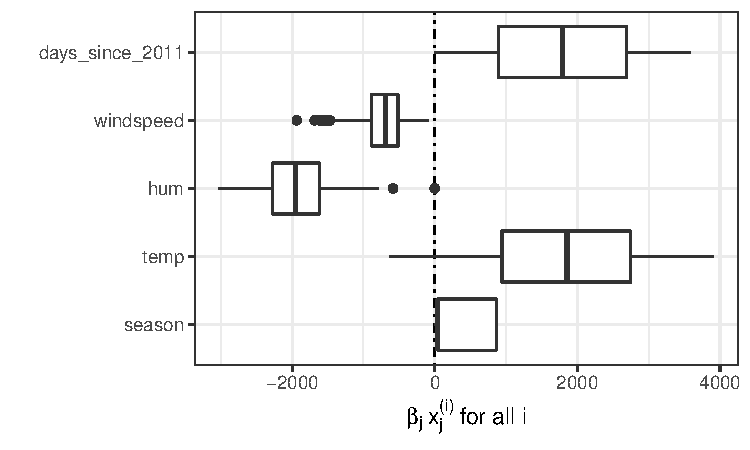
\includegraphics[width = \textwidth]{figure/plot_lin_effect.pdf}
  \begin{center}
   % Effect of $i$-th observation $= \beta_j x_j^{(i)}$\\
    $\leadsto$ Better comparability due to different scales
  \end{center}
   
\end{column}
\end{columns}
\end{frame}


\begin{frame}{Linear Regression - Example: Including Interactions}
\textbf{Update}: Add interaction between temperature and season and visualize marginal effect of temperature% with (right) and without (left) interaction.
\begin{columns}[T]
\begin{column}{0.25\textwidth}
\begin{tiny}
\begin{table}[ht]
\centering
\begin{tabular}{rr}
  \hline
 & Weights \\ 
  \hline
(Intercept) & 3453.88 \\ 
  seasonSPRING & 1317.00 \\ 
  seasonSUMMER & 4894.10 \\ 
  seasonFALL & -114.24 \\ 
  temp & 160.46 \\ 
  hum & -37.59 \\ 
  windspeed & -61.88 \\ 
  days\_since\_2011 & 4.85 \\ 
  seasonSPRING:temp & -50.68 \\ 
  seasonSUMMER:temp & -222.02 \\ 
  seasonFALL:temp & 27.24 \\ 
   \hline
\end{tabular}
\end{table}
\end{tiny}
\end{column}
\begin{column}{0.7\textwidth}
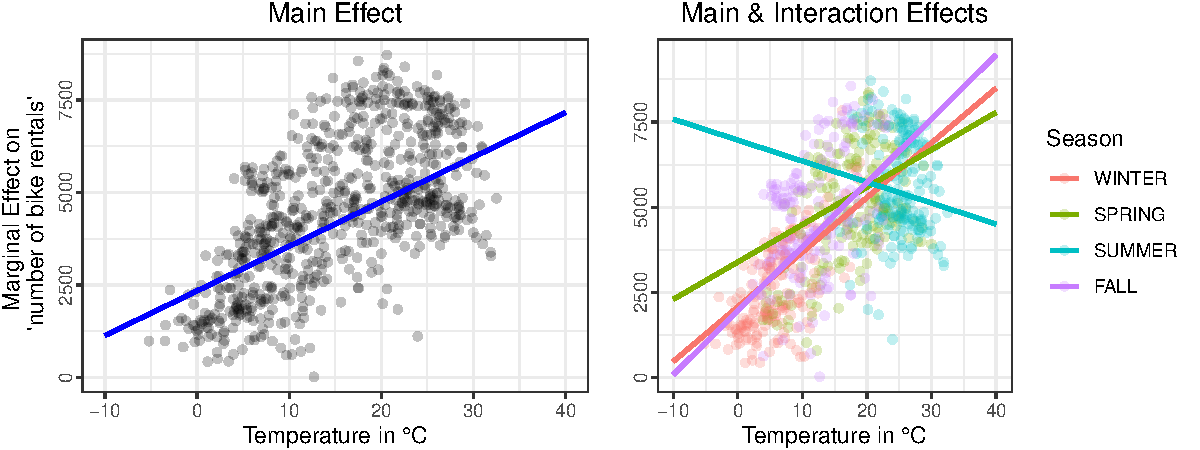
\includegraphics[width = \textwidth]{figure/lm_main_vs_interaction_effects.pdf}
\end{column}
\end{columns}
\vfill
\pause
\textbf{Interpretation}: If temperature increases by 1 degree Celsius, then number of bike rentals increases by 160 in winter and by 110 (160 + (-50)) in spring. In summer it is decreasing by -62 (160 + (-222)).\\\vspace*{0.2cm}
\textbf{Note:} Value ranges of temperature differ depending on the season $\leadsto$ not acknowledged by LM
\end{frame}


\begin{frame}{Linear Regression - Example: Including Polynomials}
\textbf{Update}: Add 2nd order polynomial for temperature to main effect (left) and main \& interaction effect (right) model.
\begin{columns}[T]
\begin{column}{0.25\textwidth}
\begin{tiny}
\begin{table}[ht]
\centering
\begin{tabular}{rr}
  \hline
 & Weights \\ 
  \hline
(Intercept) & 3094.14 \\ 
  seasonSPRING & 619.24 \\ 
  seasonSUMMER & 284.57 \\ 
  seasonFALL & 123.14 \\ 
  hum & -36.38 \\ 
  windspeed & -65.65 \\ 
  days\_since\_2011 & 4.68 \\ 
  poly(temp, 2)1 & 280.15 \\ 
  poly(temp, 2)2 & -5.58 \\ 
   \hline
\end{tabular}
\end{table}
   Table: Weights for main effect model

\end{tiny}

\end{column}
\begin{column}{0.7\textwidth}
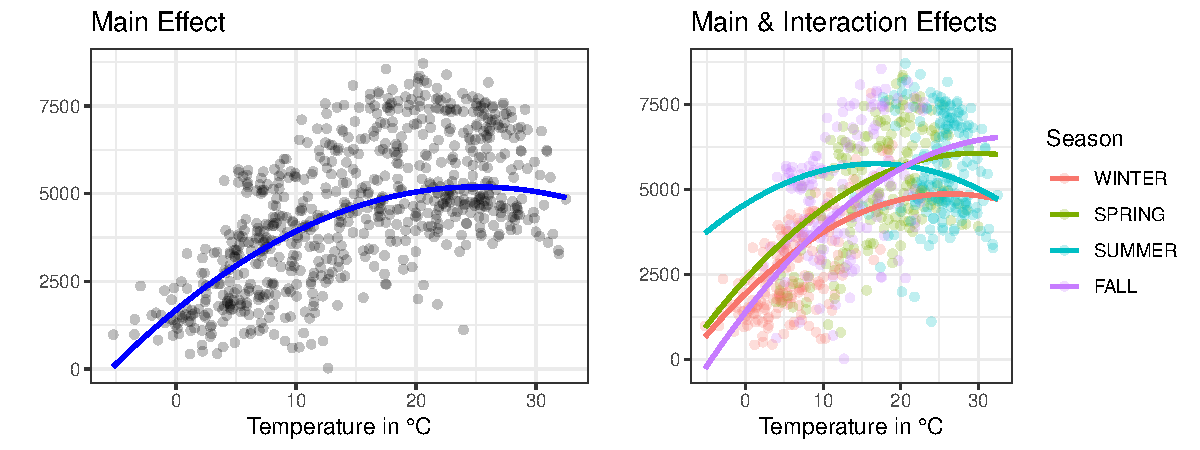
\includegraphics[width = \textwidth]{figure/poly_main_vs_interaction_effects.pdf}
\end{column}
\end{columns}
\vfill
\pause
\textbf{Interpretation}: Not linear anymore!\\ 
$\leadsto$ Effect size depends on temperature value: $280.2 \cdot temp - 5.6 \cdot temp^2$\\
$\leadsto$ BUT: Needs to be manually specified!\\
$\leadsto$ The more non-linear and interaction effects are added, the less interpretable becomes the model
\end{frame}


\begin{frame}{Sparse Linear Regression - LASSO \citebutton{Tibshirani (1996)}{https://doi.org/10.1111/j.2517-6161.1996.tb02080.x}}
\begin{itemize}
    \item Sparser models are more interpretable
    \item LASSO adds an L1-norm penalization term  ($\lambda||\beta||_1$) to the optimization problem
    \item Aim: Feature selection (sparsity) and regularization of feature weights
    \item Penalization parameter $\lambda$ must be chosen (e.g. by CV %or depending on the number of features to keep
    )
\end{itemize}


$$
min_{\beta} \bigg(\underbrace{\frac{1}{n} \sum_{i=1}^{n} (y^{(i)} - x^{(i)\top}\beta)^2}_\text{Least square estimate for LM} + \lambda||\beta||_1\bigg)
$$
\vspace*{0.2cm}\\
\textbf{Example}
\vspace*{-0.4cm}
\pause
\begin{columns}
\begin{column}{0.65\textwidth}
\begin{itemize}
    \item Penalize main effect model with polynomial term for temp
    \item $\lambda$ is chosen such that 5 features are selected
    \item May be problematic for categorical features, polynomials and interactions $\leadsto$ group LASSO \lit{Yuan and Lin (2006)}{https://doi.org/10.1111/j.1467-9868.2005.00532.x}
\end{itemize}
\end{column}
\begin{column}{0.35\textwidth}
\tiny
\begin{table}[ht]
\centering
\begin{tabular}{rr}
  \hline
 & beta \\ 
  \hline
(Intercept) & 2665.50 \\ 
  seasonSPRING & 489.34 \\ 
  seasonSUMMER & 0.00 \\ 
  seasonFALL & 0.00 \\ 
  hum & -19.44 \\ 
  windspeed & -35.54 \\ 
  days\_since\_2011 & 4.71 \\ 
  poly(temp, 2)1 & 109.25 \\ 
  poly(temp, 2)2 & 0.00 \\ 
   \hline
\end{tabular}
\end{table}
\end{column}
\end{columns}

\end{frame}
%------------------------------------------------------------------
%------------------------------------------------------------------
\begin{frame}{Generalized Linear Model (GLM) - Characteristics}

\textbf{Problem}: Target variable given the features not normally distributed $\leadsto$ LM not suitable
\begin{itemize}
    \item Target is categorical (e.g. medical diagnosis)
    \item Target is count variable (e.g. number of sold products)
    \item Time until an event occurs (e.g. time until death)
\end{itemize}
\medskip
\pause
\textbf{Solution}: GLMs - extend LMs by allowing other distributions from exponential family
$$g(\mathrm{E}_Y (y\mid x)) = \beta_0 + \beta_1 x_1 + \beta_2 x_2 + \ldots + \beta_p x_p$$
\vspace*{-0.4cm}
    \begin{itemize}
        \item Link function $g$ links weighted sum (linear predictor) to specified distribution
        \item Link function and probability distribution need to be specified by the user
        \item LM is a special case by choosing the identity function for $g$ and the Gaussian distribution
        \item Interpretation depends on specified link function and distribution
        \item Interaction and polynomial effects can be manually added in the same way as in LMs
    \end{itemize}
    
 %   \medskip
 %   Non-Gaussian outputs via Generalized Linear Models (GLMs):
    
  %  \begin{itemize}
   %     \item link function $g$ -- can be freely chosen
    %    \item exponential family defining $\mathrm{E}_Y$ -- can be freely chosen
     %   \item weighted sum $X^\top W$
    %\end{itemize}
    
    %\medskip 
    %\pause
    %Interaction effects via feature engineering:
    %\begin{itemize}
    %    \item E.g., feature expansion: $\beta_{x_i,x_j} x_i \cdot x_j$
    %\end{itemize}
    
\end{frame}
 	
\begin{frame}{Logistic Regression - Characteristics}

\begin{itemize}
    \item Logistic regression models probabilities (between 0 and 1) for binary classification tasks 
    \item GLM with Bernoulli distribution and logit link function
    \item Logistic regression formula:
    $$P(y = 1) =\frac{1}{1 + \exp(-( \beta_0 + \beta_1 x_1 + \beta_2 x_2 + \ldots + \beta_p x_p ))} $$
    \item Typically, we set the threshold to $0.5$ to predict 
        \begin{itemize}
            \item Class 1 if $P(y=1) > 0.5$
            \item Class 0 if $P(y=1) \leq 0.5$
        \end{itemize}
\end{itemize}
    

	

\end{frame}

%------------------------------------------------------------------
%------------------------------------------------------------------

\begin{frame}[c]{Logistic Regression - Interpretation}

    
    
    
    

    \begin{itemize}
        \item Weights relate to formula in log odds - again linear in log odds
        $$log\text{ }odds = \log \left(\frac{P(y = 1)}{P(y=0)}\right) = \beta_0 + \beta_1 x_1 + \beta_2 x_2 + \ldots + \beta_p x_p  $$
        \pause
        \item Odds can be caulculated by 
        $$odds = \left(\frac{P(y = 1)}{P(y=0)}\right) = \exp(\beta_0 + \beta_1 x_1 + \beta_2 x_2 + \ldots + \beta_p x_p)  $$
        \item[$\leadsto$] Change by one unit changes the odds ratio by a \alert{factor} of $\exp(\beta_J)$
        $$odds\text{ }ratio = \frac{odds_{x_j+1}}{odds} = \frac{\exp(\beta_0 + \beta_1 x_1 + \ldots + \beta_j (x_j+1) + \ldots + \beta_p x_p)}{\exp(\beta_0 + \beta_1 x_1 + \ldots + \beta_j x_j + \ldots + \beta_p x_p)} = \exp{(\beta_j)} $$
        \pause
        \item Interpretation for different feature types is the same as for linear regression (however, linear interpretation only possible for log odds $\leadsto$ difficult to comprehend)
    \end{itemize}	

\end{frame}

\begin{frame}{Logistic Regression - Example}

\begin{itemize}
    \item Create a binary target variable for bike rental data (Class 1: high number of bike rentals - more than the 70\% quantile - and Class 0: low to medium number of bike rentals)
    \item Fit a logistic regression with Bernoulli distribution and logit link
\end{itemize}

\begin{columns}[T]
\begin{column}{0.45\textwidth}
\begin{table}[ht]
\centering
\tiny
\begin{tabular}{rrrrr}
  \hline
 & Weights & Std. Error & z value & Pr($>$$|$z$|$) \\ 
  \hline
(Intercept) & -8.5 & 1.2 & -7.1 & 0.00 \\ 
  seasonSPRING & 1.7 & 0.6 & 2.9 & 0.00 \\ 
  seasonSUMMER & -0.9 & 0.8 & -1.1 & 0.26 \\ 
  seasonFALL & -0.6 & 0.6 & -1.2 & 0.25 \\ 
  temp & 0.3 & 0.0 & 7.4 & 0.00 \\ 
  hum & -0.1 & 0.0 & -5.0 & 0.00 \\ 
  windspeed & -0.1 & 0.0 & -3.0 & 0.00 \\ 
  days\_since\_2011 & 0.0 & 0.0 & 11.6 & 0.00 \\ 
   \hline
\end{tabular}
\end{table}
\pause
\textbf{Interpretation}
\begin{itemize}
    %\item If the temperature increases by 1 degree Celsius then the log odds of high number of bike rentals increase linearly by 0.3 c.p.
    \item If temperature increases by 1 degree Celsius then the odds for high number of bike rentals increase by the factor $\exp (0.3) = 1.3$ c.p.
\end{itemize}
\end{column}
\hfill
\pause
\begin{column}{0.5\textwidth}
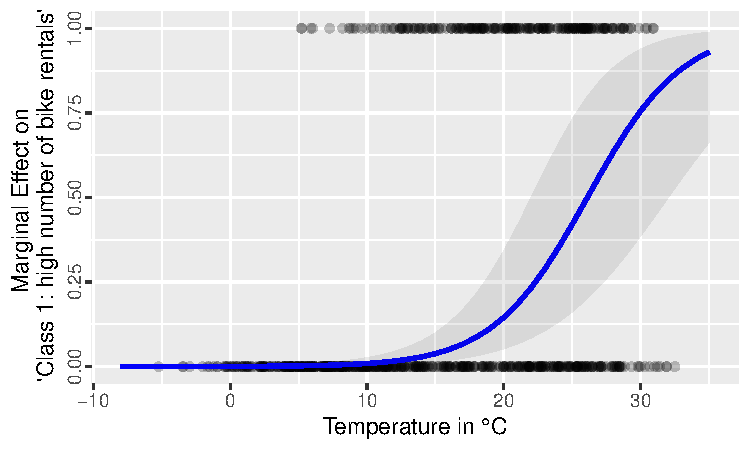
\includegraphics[width = \textwidth]{figure/logistic_maginal_temp.pdf}
\end{column}
\end{columns}

\end{frame}
%------------------------------------------------------------------
%------------------------------------------------------------------


%------------------------------------------------------------------
%------------------------------------------------------------------

\begin{frame}{Generalized Additive Models (GAMs) - Characteristics}

\textbf{Problem}: Relationship between features and target variable not linear $\leadsto$ standard LM not suitable 

\medskip
\pause
\textbf{Solution}: 
 \begin{itemize}
        \item Feature transformations (e.g., exp or log)
        \item Categorization of features (i.e., intervals / buckets of feature values)
        \item GAMs:
        $$g(\mathrm{E}_Y (y\mid x)) = \beta_0 + f_1(x_1) + f_2(x_2) + \ldots + f_p(x_p)$$
    
    \begin{itemize}
        \item Instead of $\beta_j x_j$ use flexible functions $f_j(x_j)$ $\leadsto$ splines
        \item Preserves additive structure of feature effects but does also allow nonlinear effects
        \item Smoothness parameter to control flexibility (prevent overfitting) needs to be tuned
    \end{itemize}
    \end{itemize}
    
    

   

\end{frame}


\begin{frame}{Generalized Additive Models (GAMs) - Example}
    \begin{itemize}
    \item Fit a GAM with smooth splines for four numeric features of bike rental data 
\end{itemize}

\begin{columns}[T]
\begin{column}{0.45\textwidth}
\begin{table}[ht]
\centering
\tiny
\begin{tabular}{rrrrr}
  \hline
 & edf & Ref.df & F & p-value \\ 
  \hline
s(temp) & 5.8 & 7.0 & 57.2 & 0.00 \\ 
  s(hum) & 4.0 & 5.1 & 68.0 & 0.00 \\ 
  s(windspeed) & 1.7 & 2.1 & 50.1 & 0.00 \\ 
  s(days\_since\_2011) & 8.3 & 8.8 & 154.4 & 0.00 \\ 
   \hline
\end{tabular}
\end{table}


\textbf{Interpretation}
\begin{itemize}
    %\item If the temperature increases by 1 degree Celsius then the log odds of high number of bike rentals increase linearly by 0.3 c.p.
    \item Edf (effective degrees of freedom) represents complexity of the smooth
    \item Interpretation needs to be done visually and relative to average prediction\\
    $\leadsto$ more flexibility and better model fit but less interpretability
\end{itemize}
\end{column}
\hfill
\begin{column}{0.5\textwidth}
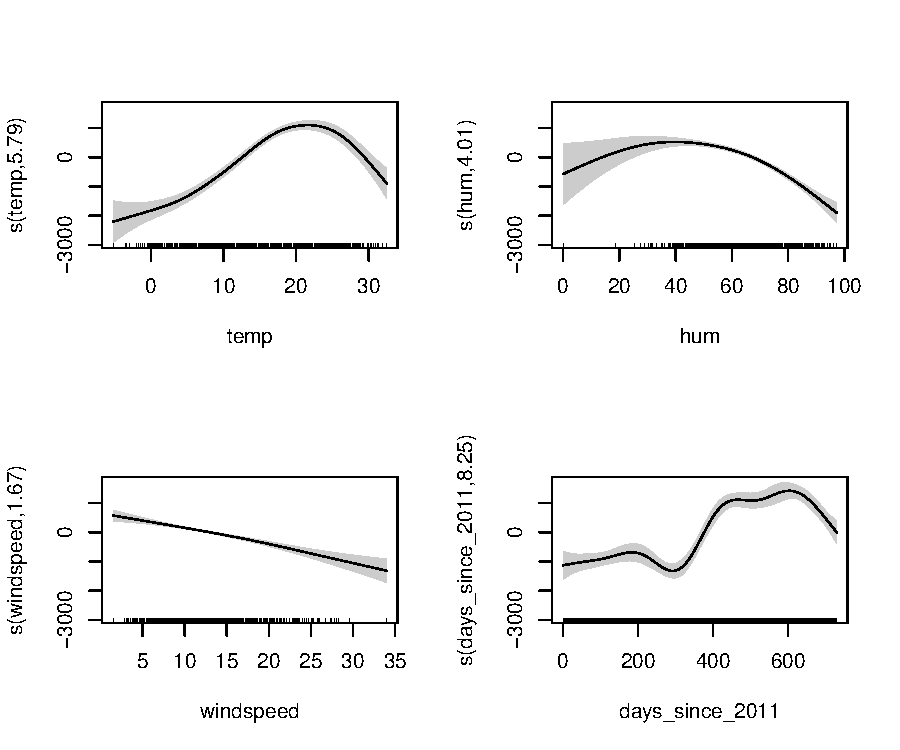
\includegraphics[width = \textwidth]{figure/gam_effects.pdf}
\end{column}
\end{columns}
\end{frame}
%------------------------------------------------------------------
%------------------------------------------------------------------

\begin{frame}{Decision Trees - Characteristics \& Interpretation}

\textbf{Problem}: Relationship between features and target are nonlinear or feature interactions are present\\
\medskip
\pause
\textbf{Solution}: Decision tree \lit{Breiman et al. (1984)}{https://doi.org/10.1201/9781315139470} -- Split data in different subsets depending on cutoff values in features 
$$
\hat f(x) = \sum_{m=1}^M c_m \mathbbm{1}_{\{x \in \mathcal{R}_m\}}\text{ ,  where $\mathcal{R}_m$ is the $m$-th leaf node of the tree}
$$

\begin{itemize}
    \item Determination of split point (CART): at split point that minimizes the variance of $y$ (regression) or the Gini index (classification)
    \item Able to handle mixed feature space
\end{itemize}
\medskip
\pause
\textbf{Interpretation}
\begin{itemize}
    \item Directly by following the tree (i.e., sequence of rules)
    \item Feature importance by (scaled) score of how much splitting criterion (e.g. variance) is reduced compared to parent
\end{itemize}



\end{frame}

\begin{frame}{Decision Trees - Example}
\begin{itemize}
    \item Fit decision tree with tree depth of 3 on bike rental data
    \item E.g., mean prediction for the first 105 days since 2011 is 1798
    \item The feature days\_since\_2011 shows highest feature importance (explains most of variance)
\end{itemize}
\begin{columns}[T]
\begin{column}{0.4\textwidth}
\begin{table}[ht]
\centering
\begin{tabular}{lr}
  \hline
Feature & Importance \\ 
  \hline
days\_since\_2011 & 68.03 \\ 
  temp & 20.54 \\ 
  season & 6.56 \\ 
  hum & 3.58 \\ 
  windspeed & 1.29 \\ 
   \hline
\end{tabular}
\end{table}
\end{column}
\begin{column}{0.6\textwidth}
  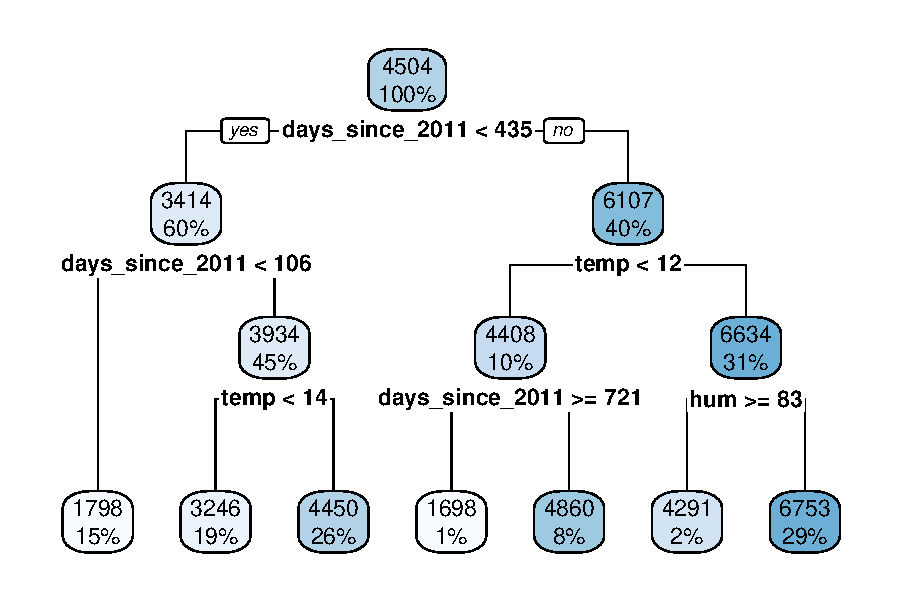
\includegraphics[width = \textwidth]{figure/tree.pdf} 
\end{column}
\end{columns}
 
\end{frame}
%------------------------------------------------------------------
%------------------------------------------------------------------

%\begin{frame}[c]{Decision Rules}

%\texttt{IF COND$_1$ AND COND$_2$ AND ... THEN value}

%\begin{itemize}
%    \item \texttt{COND$_i$} can be of the form \texttt{feature <op> value} where \texttt{<op>} can be for example $\{=, <, > \}$
%\end{itemize}

%\pause
%\medskip

%Properties:
%\begin{description}
%    \item{Support} Fraction of observations to support appliance of rule
%    \item{Accuracy} for predicting the correct class under the condition(s)
%\end{description}

%$\leadsto$ often trade-off between these two

%\pause
%\medskip

%$\leadsto$ many different ways to learn a set of rules (incl. a default rule if none of the rules are met)

%\end{frame}

%------------------------------------------------------------------
%------------------------------------------------------------------

\begin{frame}{Model-Based Boosting - Characteristics}

\begin{itemize}
%\setlength\itemsep{2em}
\item
Boosting iteratively combines weak base learners to create a powerful ensemble model
\item
Idea: Combine boosting with interpretable base learners (e.g., single feature LM) 
%The resulting ensemble is also interpretable.
\item
Two linear base learners $b_j(x, \theta)$ and $b_j(x, \theta^{\star})$ of the same type, but distinct parameter vectors $\theta$ and $\theta^{\star}$ can be combined in a base learner of the same type:
$$
b_j(x, \theta) + b_j(x, \theta^{\star}) = b_j(x, \theta + \theta^{\star})
$$
\item In each iteration, a selection of base learners is trained on pseudo residuals. The one with the best fit is added to the previously computed model:
\medskip
\begin{align*}
\widehat{f}^{[1]}(x) &= f_0 + \beta b_3(x_3, \theta^{[1]}) \\
\widehat{f}^{[2]}(x) &= f_0 + \beta b_3(x_3, \theta^{[1]}) + \beta b_3(x_3, \theta^{[2]})\\
\widehat{f}^{[3]}(x) &= f_0 + \beta b_3(x_3, \theta^{[1]}) + \beta b_3(x_3, \theta^{[2]}) + \beta b_1(x_1, \theta^{[3]}) \\
&= f_0 + \beta \left(b_3(x_3, \theta^{[1]} + \theta^{[2]}) + b_1(x_1, \theta^{[3]})\right)
\end{align*}

\item Final model has additive structure (as GAMs), where each component function is interpretable

\end{itemize}
\end{frame}


\begin{frame}{Model-Based Boosting - Characteristics \& Example}

Simplest case: Use linear models as base learners on single features
$$
b_j(x_j, \theta) = x_j\theta \hspace*{0.2cm}\text{ for } j = 1,\ldots p \hspace*{0.3cm} \leadsto \text{ordinary linear regression}
$$

\begin{itemize}
\item Converges to same solution as ML estimate
\item Specifying loss function and link function according to exponential family leads to boosting which is equivalent to a (regularized) GLM
\item Early stopping allows feature selection

\end{itemize}
\pause
\begin{columns}[T]
\begin{column}{0.4\textwidth}
\scriptsize
  \begin{table}[ht]
\centering
\begin{tabular}{rlrr}
  \hline
 Feature & Intercept & Slope \\ 
  \hline
days\_since\_2011\_linear & -1188.81 & 3.23 \\ 
 season\_ridge & -291.24 & 165.61 \\ 
 temp\_linear & -1045.34 & 70.24 \\ 
 offset & 4452.18 &  \\ 
   \hline
\end{tabular}
\end{table}
\begin{itemize}
    \item Linear base learners for numeric features and categorical base learner for season
    \item 3 base learners selected after 100 iterations
\end{itemize}
\end{column}
\begin{column}{0.55\textwidth}
  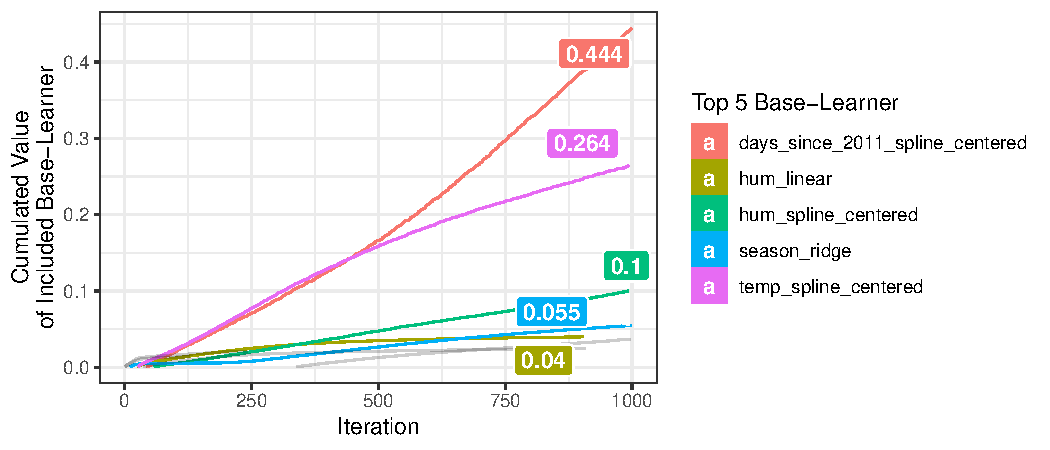
\includegraphics[width = .95 \textwidth]{figure/compboost_base_linear.pdf} 
\end{column}
\end{columns}
\end{frame}







\begin{frame}{Model-Based Boosting - Example \& Interpretation}

\begin{itemize}
    \item Fit a model-based boosting model on bike rental data \lit{Daniel Schalk et al. 2018}{https://doi.org/10.21105/joss.00967}
    \item Define base learners for all features - linear and centered splines for numeric features and categorical base learner for season
\end{itemize}
\begin{columns}[T]
\pause
\begin{column}{0.5\textwidth}
 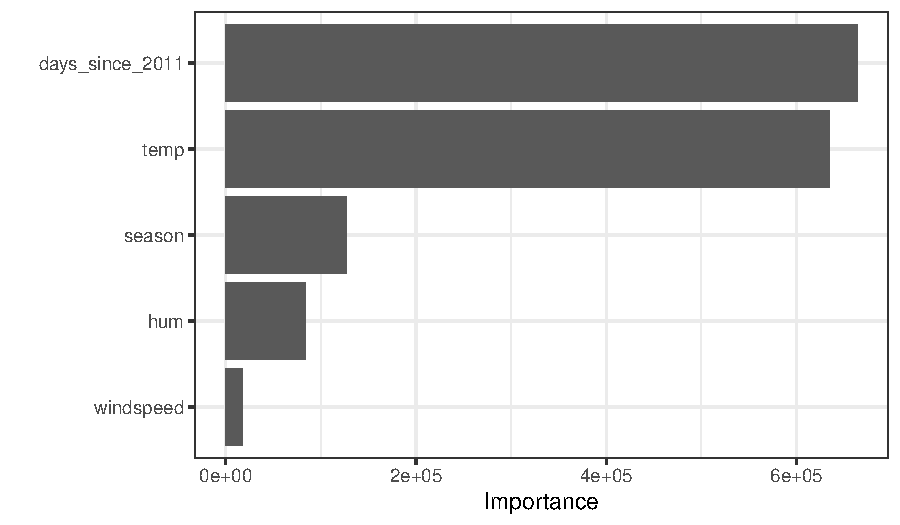
\includegraphics[width = 0.9\textwidth]{figure/compboost_pfi.pdf}
 \begin{itemize}
     \item Loss-based feature importance\\
     $\leadsto$ days\_since\_2011 is most important feature
 \end{itemize}
%\scriptsize
%\verbatiminput{figure/mboost_output.txt}
\end{column}
\pause
\begin{column}{0.5\textwidth}  %%<--- here
  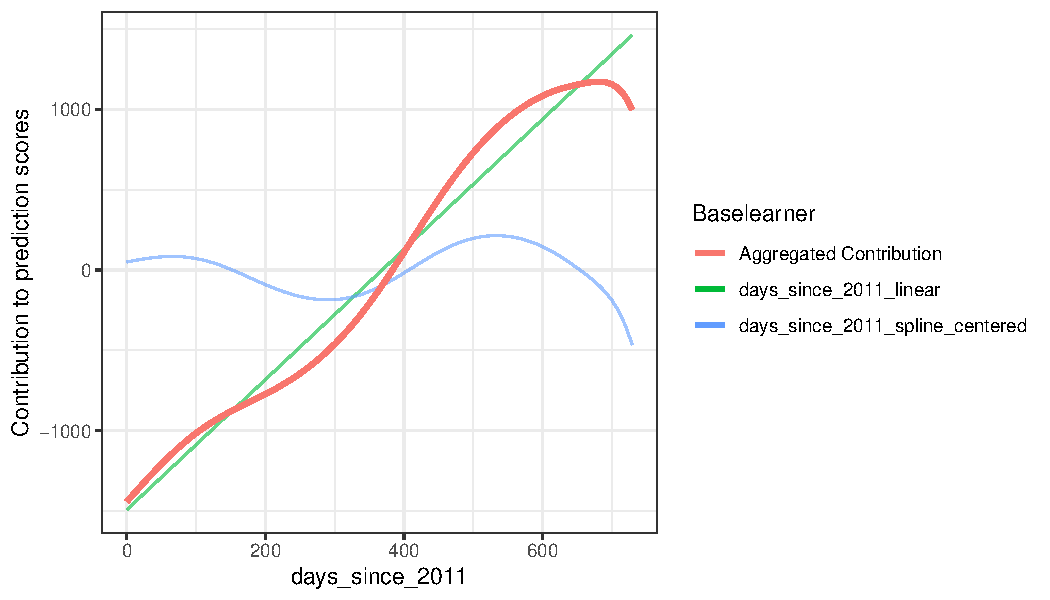
\includegraphics[width = 0.9 \textwidth]{figure/compboost_pfe.pdf}
  \begin{itemize}
      \item Partial feature effect for days\_since\_2011\\
      $\leadsto$ Total partial effect can be decomposed into partial effects of linear and centered spline base learners 
  \end{itemize}
\end{column}
\end{columns}
\end{frame}



\begin{frame}[c]{Other Interpretable Models}

\textbf{RuleFit} \lit{Friedman and Popescu 2008}{https://arxiv.org/abs/0811.1679}
\begin{itemize}
    \item Combination of linear models and decision trees 
    \item Allows for feature interactions and non-linearities
\end{itemize}

\textbf{Decision Rules} \lit{Holte 1993}{https://doi.org/10.1023/A:1022631118932}
\begin{itemize}
    \item Simple ``if -- then'' statements - very intuitive and easy-to-interpret
    \item Common assumption: only classification tasks and categorical features
\end{itemize}

\textbf{NaiveBayes}
%$$P (C_k \mid x ) = \frac{1}{Z} P(C_k) \prod_{i=1}^{n} P(x_i \mid C_k) $$
\begin{itemize}
    \item Product of probabilities for a class on the value of each feature
    \item Strong independence assumption
\end{itemize}


\textbf{k-Nearest Neighbor}
\begin{itemize}
    \item (Closely related to case-based reasoning)
    \item Average of of the outcome of neighbors -- local explanation
\end{itemize}

\end{frame}


\endlecture
\end{document}